\documentclass{article}

\usepackage{polski}
\usepackage{setspace}
\usepackage[polish]{babel}
\usepackage[utf8]{inputenc}
\usepackage{listings}

\usepackage{graphicx}
\graphicspath{ {./img/} }

\lstset{columns=fullflexible,basicstyle=\ttfamily}

\usepackage{float}
\usepackage{datetime}
\usepackage{amsmath}

\setlength\parindent{0pt}

\begin{document}

\begin{titlepage}

\newcommand{\HRule}{\rule{\linewidth}{0.5mm}} % Defines a new command for the horizontal lines, change thickness here

\center % Center everything on the page
 
%----------------------------------------------------------------------------------------
%	HEADING SECTIONS
%----------------------------------------------------------------------------------------

\textsc{\LARGE Politechnika Poznańska}\\[1.5cm] % Name of your university/college
\textsc{\Large Wydział Informatyki}\\[0.5cm] % Major heading such as course name
\textsc{\large Przetwarzanie Równoległe}\\[0.5cm] % Minor heading such as course title

%----------------------------------------------------------------------------------------
%	TITLE SECTION
%----------------------------------------------------------------------------------------

\HRule \\[0.4cm]
{ \huge \bfseries Optymalizacja przetwarzania równoległego}\\[0.4cm] % Title of your document
\HRule \\[1.5cm]
 
%----------------------------------------------------------------------------------------
%	AUTHOR SECTION
%----------------------------------------------------------------------------------------

\begin{minipage}[t]{0.4\textwidth}
\begin{flushleft} \large
\emph{Autorzy:}\\
Adam \textsc{Szczepański} \\
Mateusz \textsc{Czajka} % Your name
\end{flushleft}
\end{minipage}
~
\begin{minipage}[t]{0.4\textwidth}
\begin{flushright} \large
\emph{Prowadzący:} \\
dr Rafał \textsc{Walkowiak} % Supervisor's Name
\end{flushright}
\end{minipage}\\[2cm]

%----------------------------------------------------------------------------------------
%	LOGO SECTION
%----------------------------------------------------------------------------------------

\begin{figure}[h]
\centering

\includegraphics[width=0.4\textwidth]{PUT_logo.png}\\[1cm] % Include a department/university logo - this will require the graphicx package
\end{figure}

%----------------------------------------------------------------------------------------
%	DATE SECTION
%----------------------------------------------------------------------------------------

{\large \today}\\[1cm] % Date, change the \today to a set date if you want to be precise

 
%----------------------------------------------------------------------------------------

\vfill % Fill the rest of the page with whitespace

\end{titlepage}


\tableofcontents
\newpage

\section{Informacje o projekcie}

\subsection{Dane autorów}

\begin{center}
\begin{tabular}{l r}
Mateusz Czajka & 106596 \\
Adam Szczepański & 106593
\end{tabular}
\end{center}

\subsection{Historia projektu}

\newdate{first-ver-date}{20}{01}{2013}

\begin{center}
\begin{enumerate}
\item Jest to pierwsza wersja projektu. Dokumentacja elektroniczna została przesłana w dniu \displaydate{first-ver-date}.
\end{enumerate}
\end{center}

\newpage
\section{Wprowadzenie}

Celem projektu było zapoznanie się z możliwościami przetwarzania na kartach graficznych na przykładzie technologi CUDA.\\
Przygotowaliśmy 6 wersji programu, którego zadaniem było mnożenie macierzy kwadratowych na GPU:
\begin{enumerate}
\item wykorzystanie 1 bloku wątków
\item wykorzystanie gridu wieloblokowego wątków
\item wykorzystanie gridu wieloblokowego wątków i pamięci współdzielonej
\item wykorzystanie gridu wieloblokowego wątków i pamięci współdzielonej, zrównoleglone pobranie danych i obliczenia
\begin{enumerate}[(a)]
\item pobranie danych do rejestru
\item pobranie danych do pamięci współdzielonej
\end{enumerate}
\item wykorzystanie gridu wieloblokowego wątków i pamięci współdzielonej, zrównoleglone pobranie danych i obliczenia, powiększona ilość pracy każdego wątku
\end{enumerate}

Dla każdej wersji podajemy teoretyczną zajętość SM warpami wynikającą z rozmiaru bloku, wykorzystanej liczby rejestrów, rozmiaru pamięci współdzielonej, a także z ograniczeń GPU\@. Wyjątkiem jest wersja 1. w której wykorzystany jest tylko 1 blok, zatem zajętość SM wynika tylko z jego rozmiaru.\\
W przypadku pozostałych wersji, dla poszczególnych parametrów podany jest w tabeli limit bloków -- oznacza on ile bloków maksymalnie można powiązać z SM przy danych parametrach. Jeśli wszystkie limity są większe od limitu bloków na SM wynikającego z ograniczeń GPU, to limit bloków GPU determinuje ilość aktywnych bloków, a co za tym idzie zajętość SM.\\
Efektywność programów zbadaliśmy także przy pomocy profilera NVIDIA Visual Profiler. Dla każdej instancji podajemy:
\begin{itemize}
\item czas wykonania
\item ilość operacji zmiennoprzecinkowych na sekundę (GFLOPS)
\item ilość instrukcji wykonanych na sekundę (GIPS)
\item stosunek operacji zmiennoprzecinkowych do ilości operacji odczytu/zapisu z pamięci globalnej (CGMA)
\end{itemize}

Ze względu na zupełnie odmienne podejścia w wersjach 1, 2 i 3, oraz modyfikacje wersji 3. w wersjach 4a, 4b i 5 rozmiary macierzy i bloków podzieliliśmy na dwie grupy:
\begin{itemize}
\item Wersje 1, 2 i 3 -- macierze 176x176, 352x352 oraz 528x528, bloki 8x8, 16x16, 22x22 (wymiary macierzy są podzielne przez 8, 16 i 22).
\item Wersje: 3, 4a, 4b, 5  -- macierze 128x128, 256x256, 384x384, 512x512, 640x640, bloki 8x8, 16x16 (wymiary macierzy podzielne przez 16 i 32).
\end{itemize}

Na zakończenie prezentujemy porównanie efektywności wszystkich badanych wersji.

\section{Pomiary efektywności}

\subsection{Przyśpieszenie obliczeń równoległych}

\subsubsection{Pomiary}

\begin{table}[!ht]
\caption{Porównanie szybkości wybranych algorytmów wobec $sum\_ij$}
\begin{tabular}{|c|c|c|}

\hline
  Algorytm &
  Czas wykonania w $ms$ &
  Przyśpieszenie względem $sum\_ij$ \\

\hline
  $sum\_ij$ &
  253 &
  1.000 \\

\hline
  $sum\_ji$ &
  2362 &
  0.107 \\

\hline
  $sum\_par\_ij$ &
  87 &
  2.908 \\

\hline
  $sum\_par\_ji$ &
  1189 &
  0.213 \\

\hline

\end{tabular}
\end{table}

Warto zwrócić uwagę na fakt, że oprócz braku lub obecności zrównoleglenia znaczący wpływ na szybkość przetwarzania ma kolejność uszeregowania pętli. Zostało to szerzej omówione w sekcji \ref{sec:trafienia}. Przyśpieszenia dla poszczególnych uszeregowań pętli prezentują się następująco:

\begin{table}[!ht]
\caption{Porównanie szybkości wybranych algorytmów (o kolejności pętli $ij$) wobec $sum\_ij$}
\begin{tabular}{|c|c|c|}

\hline
  Algorytm &
  Czas wykonania w $ms$ &
  Przyśpieszenie względem $sum\_ij$ \\

\hline
  $sum\_ij$ &
  2362 &
  1.000 \\

\hline
  $sum\_par\_ij$ &
  87 &
  2.908 \\

\hline

\end{tabular}
\end{table}

\begin{table}[!ht]
\caption{Porównanie szybkości wybranych algorytmów (o kolejności pętli $ji$) wobec $sum\_ji$}
\begin{tabular}{|c|c|c|}

\hline
  Algorytm &
  Czas wykonania w $ms$ &
  Przyśpieszenie względem $sum\_ji$ \\

\hline
  $sum\_ji$ &
  2362 &
  1.000 \\

\hline
  $sum\_par\_ji$ &
  1189 &
  1.987 \\

\hline

\end{tabular}
\end{table}

\subsubsection{Podsumowanie}

Zrównoleglenie przetwarzania znacząco przyśpiesza jego czas przetwarzania. Znaczeny wpływ na wielkość wartości tego przyśpieszenia ma kolejność uszeregowania pętli. W przybliżeniu jest to:
\begin{itemize}
\item trzykrotne przyśpieszenie dla uszeregowania pętli $ij$
\item dwukrotne przyśpieszenie dla uszeregowania pętli $ji$
\end{itemize}

\subsection{Ilość wykonanych instrukcji na jeden cykl procesora}

IPC (insructions per cycle) jest jednym z wyznaczników prędkości procesora. Oznacza on liczbę wykonywanych instrukcji przez procesor w jednym cyklu zegara. Wskaźnik IPC obliczaliśmy dla każdej funkcji na podstawie wzoru:
\begin{equation}
  IPC = \frac{ret\_instr}{CPU\_clocks}.
\end{equation}

CPI (cycles per instruction) jest odwrotnością CPI:
\begin{equation}
  CPI = \frac{CPU\_clocks}{ret\_instr}.
\end{equation}

\begin{table}[!ht]
\caption{Wartości IPC i CPI dla poszczególnych algorytmów}
\begin{tabular}{|c|c|c|c|c|}

\hline
  Algorytm &
  $ret\_instr$ &
  $CPU\_clocks$ &
  $IPC$ &
  $CPI$ \\

\hline
  $sum\_ij$ &
  12640 &
  14736 &
  0.86 &
  1.17 \\

\hline
  $sum\_ji$ &
  9780 &
  136048 &
  0.07 &
  13.91 \\

\hline
  $sum\_par\_ij$ &
  12684 &
  20096 &
  0.63 &
  1.58 \\

\hline
  $sum\_par\_ji$ &
  11524 &
  259628 &
  0.04 &
  22.53 \\

\hline
  $sum\_sec$ &
  14420 &
  1139472 &
  0.01 &
  79.02 \\

\hline
  $sum\_pf$ &
  14996 &
  13140 &
  1.14 &
  0.88 \\

\hline

\end{tabular}
\end{table}

Zgodnie z oczekiwaniami najwyższe wartości wzkaźnika IPC (a zarazem najniższe CPI) wysętpują w przypadku algorytmów, które spełniają zasadę lokalności przestrzennej, są to:
\begin{itemize}
\item $sum\_ij$
\item $sum\_par\_ij$
\item $sum\_pf$
\end{itemize}

IPC dla wyżej wymienionej grupy algorytmów jest kilkunasto a w niektórych przypadkach kilkudziesiącio krotonie większe niż dla algorytmów z pozostałej grupy.

\subsection{Współczynniki braku trafień do pamięci}
\label{sec:trafienia}

\subsubsection{Znaczenie danych}

\begin{table}[H]
\caption{Badane dane}
\begin{tabular}{|l|l|}

\hline
  Nazwa &
  Znaczenie \\
\hline
  DC acceesses &
  ilość odwołań do pamięci podręcznej \\
\hline
  DC misses &
  ilość chybień do pamięci podręcznej \\
\hline
  L2 requests &
  ilość odwołań do pamięci L2 \\
\hline
  L2 misses &
  ilość chybień do pamięci L2 \\
\hline
  L2 fill write &
  zapis danych w L2 powodowany usunięciem ich z pp L1 \\
\hline
  DRAM accesses &
  ilość odwołań do pamięci dynamicznej \\
\hline

\end{tabular}
\end{table}


\subsubsection{Pomiary}

Wartości $DC\_accesss$ oraz $DC\_missess$ odczytaliśmy bezpośrednio z programu CodeAnalyst. Natomiast $DC\_miss\_ratio$ oraz $DC\_miss\_rate$ obliczyliśmy w następujący sposób:

\begin{equation}
  DC\_miss\_rate = \frac{DC\_missess}{ret\_instr}
\end{equation}

\begin{equation}
  DC\_miss\_ratio = \frac{DC\_missess}{DC\_accesss}
\end{equation}

\begin{table}[H]
\caption{Pomiary związane z odwołaniami do pamięci L1}

\begin{tabular}{|l|c|c|c|c|}

\hline
  Algorytm &
  DC accessess &
  DC missess &
  DC miss ratio &
  DC miss rate \\

\hline
  $sum\_ij$ &
  5792 &
  24 &
  $0\%$ &
  $0\%$ \\

\hline
  $sum\_ji$ &
  7620 &
  4068 &
  $53\%$ &
  $42\%$ \\

\hline
  $sum\_par\_ij$ &
  5188 &
  20 &
  $0\%$ &
  $0\%$ \\

\hline
  $sum\_par\_ji$ &
  7652 &
  4456 &
  $58\%$ &
  $38\%$ \\

\hline
  $sum\_sec$ &
  18808 &
  5256 &
  $28\%$ &
  $36\%$ \\

\hline
  $sum\_pf$ &
  9928 &
  24 &
  $0\%$ &
  $0\%$ \\

\hline

\end{tabular}

\end{table}

Podobnie jak w przypadku pamięci L1 wartości $L2\_requests$, $L2\_misses$ oraz $L2\_fill\_write$ odczytaliśmy bezpośrednio z programu CodeAnalyst. Natomiast $L2\_miss\_ratio$ oraz $L2\_miss\_rate$ obliczyliśmy w następujący sposób:

\begin{equation}
  L2\_miss\_rate = \frac{L2\_missess}{ret\_instr}
\end{equation}

\begin{equation}
  L2\_miss\_ratio = \frac{L2\_missess}{L2\_requests + L2\_fill\_write}
\end{equation}

\begin{table}[H]
\caption{Pomiary związane z odwołaniami do pamięci L2}

\begin{tabular}{|l|c|c|c|c|c|}

\hline
  Algorytm &
  L2 requests &
  L2 missess &
  L2 fill write &
  L2 miss rate &
  L2 miss ratio \\

\hline
  $sum\_ij$ &
  663 &
  340 &
  684 &
  $3\%$ &
  $25\%$ \\

\hline
  $sum\_ji$ &
  5452 &
  7209 &
  10908 &
  $56\%$ &
  $30\%$ \\

\hline
  $sum\_par\_ij$ &
  1431 &
  352 &
  668 &
  $3\%$ &
  $17\%$ \\

\hline
  $sum\_par\_ji$ &
  5472 &
  23736 &
  10844 &
  $47\%$ &
  $16\%$ \\

\hline
  $sum\_sec$ &
  11024 &
  15945 &
  21668 &
  $76\%$ &
  $29\%$ \\

\hline
  $sum\_pf$ &
  344 &
  693 &
  684 &
  $2\%$ &
  $25\%$ \\

\hline

\end{tabular}

\end{table}

\section{Wpływ rozmiaru danych}

\subsection{Wstęp}

W celu sprawdzenia wpływu rozmiaru danych na czas realizacji zadania dokonaliśmy pomiarów czasów dla dwóch rozmiarów danych:

\begin{itemize}
\item Instancja A: $tab[2^{24}][2^4]$
\item Instancja B: $tab[2^{22}][2^4]$
\end{itemize}

Spodziewaliśmy się, że czas obliczeń dla Instancji B będzie w przybliżeniu czterokrotnie krótszy.

\subsection{Wyniki}

Wyniki pomiarów prezentują się następująco:

\begin{table}[H]
\centering
\begin{tabular}{|c|c|c|c|c|c|c|}
\hline
Problem & $sum\_ij$ & $sum\_ji$ & $sum\_sec$ & $sum\_pf$ & $sum\_par\_ij$ & $sum\_par\_ji$ \\ \hline
Instancja A & 253 & 2352 & 19552 & 225 & 87 & 1189 \\ \hline
Instancja B & 62 & 590 & 4890 & 57 & 23 & 304 \\ \hline
Stosunek A/B & 4.081 & 4.003 & 3.998 & 3.947 & 3.783 & 3.911 \\ \hline
\end{tabular}
\caption{Czas realizacji kodu dla poszczególnych funkcji w $ms$.}
\end{table}

\subsection{Podsumowanie}

Wyniki eksperymentu są bardzo zadowalające. W przypadku każdego algorytmu rozmiar danych ma liniowy wpływ na czas przetwarzania. Jest to zgodne ze złożonością algorytmu która jest liniowa wobec $n$ gdzie $n$ to $liczba\_wierszy * liczba\_kolumn$.\newline

W każdym przypadku czas realizacji dla Instancji B był około $4$ razy krótszy niż dla Instancji A. Średnia tych wartości wynosi $3.954$.

\section{Wpływ sekcyjności pamięci}

\subsection{Wstęp}

W trakcie naszych badań sprawdziliśmy wpływ sekcyjności pamięci na czas przetwarzania. Kluczowe dla tego podpunktu algorytmy to:

\begin{itemize}
\item $sum\_ij$ - podstawowy algorytm sekwencyjny, służący jako punkt odeniesienia
\item $sum\_sec$ - algorytm sekwencyjny w którym badaliśmy sekcyjność pamięci
\end{itemize}

W wykorzystywanym systemie długość lini PP wynosi $64B$, a liczba lini w pojedyńczej stronie wynosi $512$.\newline

W metodzie $sum\_sec$ w kolejnych iteracjach odwołujemy się do komórki tabeli z tej samej kolumny, z wiersza przesuniętego o ilość lini w stronie. Powoduje to konieczność wymiany całej lini PP w każdej iteracji.

\subsection{Wyniki}

Zgodnie z założeniem, powinien to być najwolniejszy algorytm, ponieważ spodziewana jest bardzo wysoka liczba odwołań do pamięci RAM or wysoki stosunek braku trafień do pamięci podręcznej.

\begin{table}[H]
\centering
\begin{tabular}{|l|c|c|c|c|}
\hline
Algorytm & Czas [ms] & DC missess & L2 misses & DRAM access \\ \hline
$sum\_ij$ & 253 & 24 & 340 & 352 \\ \hline
$sum\_sec$ & 19552 & 5256 & 11024 & 5920 \\ \hline
\end{tabular}
\caption{Porównanie wybranych algorytmów pod kątem sekcyjności pamięci}
\end{table}

Wyniki przerosły nasze oczekiwania - $sum\_sec$ wykonał się ponad $77$ razy wolniej. Pokazuje to jest wielkie znaczenie na szybkość realizacji przetwarzania ma zachowanie cechy lokalności przestrzennej. Wyraźnie widać, że w przypadku algorytmu użytego jako punkt odniesienia liczba braków trafień do pamięci podręcznej L1 była znacznie mniejsza. Sytuacja wygląda bardzo podobnie dla pamięci podręcznej L2. Konsekwencją braku trafień do pamięci podręcznej jest konieczność większej liczby pobrań danych z pamięci dynamicznej co odzwierciedla współczynnik $DRAM\_accesses$.

\section{Wyprzedzające pobranie danych}

Wyprzedzające pobranie danych potraktowaliśmy jako swego rodzaju eksperyment. Nasze obawy związane z optymlizacją kody okazały się być uzasadnione. W celu realizacji problemu dodaliśmy zmienną $tmp$, na której nie były realizowane żadne operacje. Eksperyment podzieliliśmy na dwie części.

\subsection{Klasyczne podejście}

Początkowo spodziewaliśmy się, że kompilator usunie nic nie robiące przepisanie. Po przejrzeniu instrukcji Assemblera okazało się, że jest inaczej.

\begin{figure}[!ht]
\centering
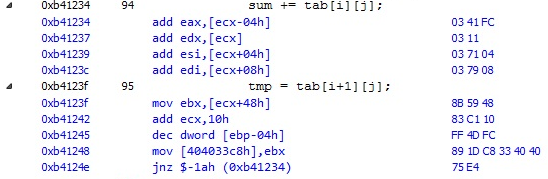
\includegraphics[width=0.5\textwidth]{pf.png}
\caption{Instrukcja przypisania do zmiennej $tmp$}
\label{fig:symetry}
\end{figure}

\begin{table}[H]
\caption{Czasy algorytmów kluczowych dla wyprzedzającego pobrania}

\begin{tabular}{|l|c|}

\hline
  Algorytm &
  Czas [ms] \\

\hline
  $sum\_ij$ &
  253 \\

\hline
  $sum\_pf$ &
  225 \\

\hline

\end{tabular}

\end{table}

Przyśpieszenie związane z wyprzedzającym pobraniem danych okazało się jednak być bardzo nieznaczne.

\subsection{Zastosowanie kwalifikatora $volatile$}

$volatile$ w C++ jest kwalifikatorem typu informującym kompilator, ze wartość zmiennej może się zmienić bez jego wiedzy i kontroli i że w związku z tym kompilator powinien zrezygnować z agresywnej optymalizacji i przy każdym odwołaniu do tej zmiennej wczytać nową wartość z komórki pamięci.\newline

Kod odpowiedzialny za inicjalizację zmiennej $tmp$ prezentował się następująco:

\lstinputlisting{./code/volatile.cpp}

Zastosowanie wyżej wymienionego kwalifikatora spowodowało zgodnie z oczekiwaniami pogorszenie czasu przetwarzania.




\section{Podsumowanie}

Zrealizowane zadania pozwoliły nam na lepsze poznanie przetwarzania równoległwego a także wagi kolejności odwołań do pamięci. Dwa główne wnioski jakie można wyciągnąć to:

\begin{itemize}
\item przetwarzanie równoległe jest szybsze od sekwencyjnego (doskonale widać poprzez porównanie algorytmów $sum\_ij$ oraz $sum\_par\_ij$)
\item ważne podczas pisania kodu jest zaplanowanie dostępów do pamięci, zapewnienie własności lokalności czasowej i przestrzennej w znaczący sposób przyspiesza działanie progoramu ($sum\_ij$ 77 krotnie szybszy od $sum\_sec$)
\end{itemize}

Najszybszy algorytm ($sum\_par\_ij$) był blisko 225 razy szybszy od najwolniejszego ($sum\_sec$). Było dla nas sporym zaskoczeniem, że takie różnice można uzyskać dla wydawało by się zwykłego sumowania komórek z tablicy.\newline

Dodatkowo warto zauważyć, że rozmiar danych liniowo (w naszym przypadku) ogranicza czas wykonania programu niezależnie czy obliczenia są wykonywane równolegle czy sekwencyjnie.


\section{Załączniki}

\begin{enumerate}
\item sekwencyjny1.lp -- plik z testem~\ref{test1}
\item sekwencyjny2.lp -- plik z testem~\ref{test2}
\item sekwencyjny3.lp -- plik z testem~\ref{test3}
\item rownolegly1.lp -- plik z testem~\ref{test4}
\item rownolegly2.lp -- plik z testem~\ref{test5}
\end{enumerate}

\newpage

\section{Kod źródłowy}

\lstinputlisting[caption=Cały program., numbers=left]{./code/sum.cpp}





\listoffigures
\addcontentsline{toc}{section}{Spis rysunków}
\listoftables
\addcontentsline{toc}{section}{Spis tablic}


\end{document}
